\documentclass[mathNotesPreamble]{subfiles}
\begin{document}
\relscale{1.4} %TODO
\section{17.4: Green's Theorem}

  \begin{thmBox*}[Green's Theorem --- Circulation Form]
    Let $C$ be a simple closed piecewise-smooth curve, oriented counterclockwise, that encloses a connected and simply connected regin $R$ in the plane. Assume $\mathbf F=\bracket{f,g}$, where $f$ and $g$ have continuous first partial derivatives in $R$. Then
      \[\underbrace{\oint_C \mathbf F\cdot d\vecr}_{\textcolor{blue}{\textnormal{circulation}}}=\underbrace{\oint_C f\,dx+g\,dy}_{\textcolor{blue}{\textnormal{circulation}}}=\iint\limits_R\parens{\frac{\partial g}{\partial x}-\frac{\partial f}{\partial y}}\,dA.\]
  \end{thmBox*}

  \begin{flushright}
    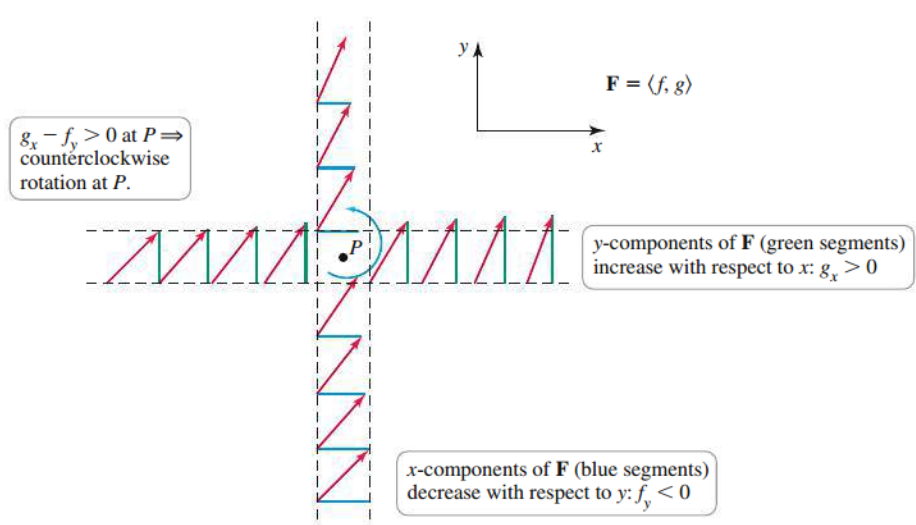
\includegraphics[width=0.825\linewidth]{images/briggs_17_04/fig17_32}
  \end{flushright}

  \begin{defn*}[Two-Dimensional Curl]
    The \textbf{two-dimensional curl} of the vector field $\mathbf F=\bracket{f,g}$ is $\displaystyle \frac{\partial g}{\partial x}-\frac{\partial f}{\partial y}$. If the curl is zero throughout a region, the vector field is \textbf{irrotational} on the region.
  \end{defn*}
  \pagebreak

  \noindent
  \begin{ex*}
    Consider the following vector fields $\mathbf F$ over the region $R=\set{(x,y): x^2+y^2\leq 1}$. Compute the circulation using Green's Theorem.
  \end{ex*}
  
  \begin{tasks}[after-item-skip=\stretch{1}, label=](1)
    \task 
      $\mathbf F=\bracket{-y, x}$\\
      \begin{flushright}
        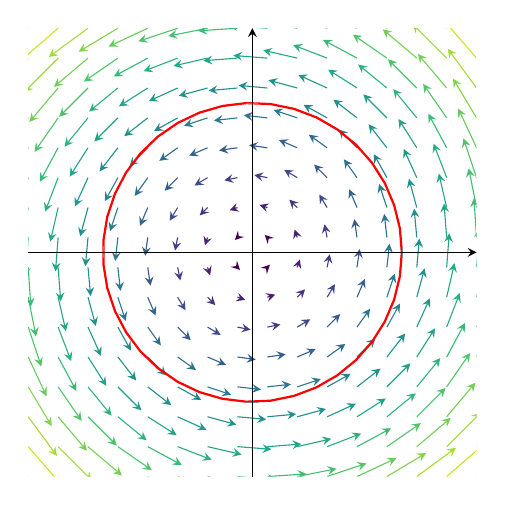
\begin{tikzpicture}
          \begin{axis}[
            	xmin = -1.5, xmax = 1.5,
            	ymin = -1.5, ymax = 1.5,
            	zmin = 0, zmax = 1,
            	axis equal image,
            	axis lines =center,
            	xtick distance = 1,
            	ytick distance = 1,
            	xticklabels={},
            	yticklabels={},
            	view = {0}{90},
            	colormap/viridis,
             ]
             \addplot3[
               point meta = {sqrt(x^2+y^2)},
               quiver = {
               u = -y,
               v = x,
               scale arrows = 0.175,
               },
               quiver/colored = {mapped color},
               samples=16,
               -stealth,
               domain = -1.5:1.5,
               domain y = -1.5:1.5,] {0};
              \draw [red, thick,  domain=0:2*pi, samples=40] 
                plot ({cos(deg(\x))}, {sin(deg(\x))} );
          \end{axis}
        \end{tikzpicture}
      \end{flushright}

    \task 
      $\mathbf F=\bracket{x, y}$\\
      \begin{flushright}
        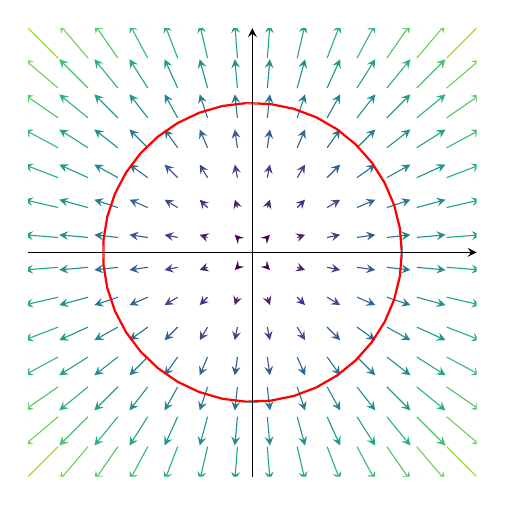
\begin{tikzpicture}
          \begin{axis}[
            	xmin = -1.5, xmax = 1.5,
            	ymin = -1.5, ymax = 1.5,
            	zmin = 0, zmax = 1,
            	axis equal image,
            	axis lines =center,
            	xtick distance = 1,
            	ytick distance = 1,
            	xticklabels={},
            	yticklabels={},
            	view = {0}{90},
            	colormap/viridis,
             ]
             \addplot3[
               point meta = {sqrt(x^2+y^2)},
               quiver = {
               u = x,
               v = y,
               scale arrows = 0.175,
               },
               quiver/colored = {mapped color},
               samples=16,
               -stealth,
               domain = -1.5:1.5,
               domain y = -1.5:1.5,] {0};
              \draw [red, thick,  domain=0:2*pi, samples=40] 
                plot ({cos(deg(\x))}, {sin(deg(\x))} );
          \end{axis}
        \end{tikzpicture}
      \end{flushright}
  \end{tasks}
  \vspace*{\stretch{1}}
  \pagebreak

  \begin{thmBox*}[Area of a Plane Region by Line Integrals]
    Under the conditions of Green's Theorem, the area of a region $R$ enclosed by a curve $C$ is
      \[\oint_C x\,dy=-\oint_C y\,dx=\frac{1}{2}\oint_C\parens{x\,dy-y\,dx}.\]
  \end{thmBox*}

  \begin{ex*}
    Find the area of the ellipse $\displaystyle \frac{x^2}{a^2}+\frac{y^2}{b^2}=1$.
  \end{ex*}
  \vspace*{\stretch{1}}
  \pagebreak

  \begin{thmBox*}[Green's Theorem --- Flux Form]
    Let $C$ be a simple closed piecewise-smooth curve, oriented counterclockwise, that encloses a connected and simply connected region $R$ in the plane. Assume $\mathbf F=\bracket{f,g}$, where $f$ and $g$ have continuous first partial derivatives in $R$. Then
      \[\underbrace{\oint_C \mathbf F\cdot \vecn ds}_{\textcolor{blue}{\textnormal{outward flux}}}=\underbrace{\oint_C f\,dy-g\,dx}_{\textcolor{blue}{\textnormal{outward flux}}}=\iint\limits_R\parens{\frac{\partial f}{\partial x}+\frac{\partial g}{\partial y}}\,dA,\]
    where $\vecn$ is the outward unit normal vector on the curve.
  \end{thmBox*}

  \begin{defn*}[Two-Dimensional Divergence]
    The \textbf{two-dimensional divergence} of the vector field $\mathbf F=\bracket{f,g}$ is $\displaystyle \frac{\partial f}{\partial x}+\frac{\partial g}{\partial y}$. If the divergence is zero throughout a region, the vector field is \textbf{source free} on that region.
  \end{defn*}

  \begin{center}
    \renewcommand{\arraystretch}{2.5}
    \begin{tabularx}{0.95\linewidth}{@{}X@{\hspace*{60pt}}X@{}}
      \textbf{Conservative Fields $\mathbf F=\bracket{f,g}$}& \textbf{Source-Free Fields $\mathbf F=\bracket{f,g}$}\\\midrule
      %
      curl $\ds = \frac{\partial g}{\partial x}-\frac{\partial f}{\partial y}=0$& 
      divergence $\ds = \frac{\partial f}{\partial x}+\frac{\partial g}{\partial y}=0$\\
      %
      Potential function $\varphi$ with \newline
      $\mathbf F=\grad\varphi$\hfill or\hfill $\ds f=\frac{\partial \varphi}{\partial x}$,\hfill $\ds g=\frac{\partial \varphi}{\partial y}$& 
      Stream function $\psi$ with 

      $\ds f=\frac{\partial \psi}{\partial y}$, \hspace*{25pt} $\ds g=-\frac{\partial \psi}{\partial x}$\\
      %
      Circulation $\ds=\oint_C \mathbf F\cdot d\vecr=0$ on all
      
      closed curves $C$.& 
      Flux $\ds=\oint_C \mathbf F\cdot\vecn\,ds=0$ on all closed curves $C$.\\
      %
      Evaluation of the line integral \newline$\displaystyle \int_C \mathbf F\cdot d\vecr = \varphi(B)-\varphi(A)$&
      Evaluation of the line integral \newline$\displaystyle \int_C \mathbf F\cdot \vecn\,ds = \psi(B)-\psi(A)$\\\bottomrule
    \end{tabularx}
  \end{center}
  \pagebreak

  \begin{center}
    \renewcommand{\arraystretch}{1.75}
    \begin{tabularx}{\linewidth}{@{}
      >{\hsize=0.8\hsize}X
      >{\hsize=1.1\hsize}X
      >{\hsize=1.1\hsize}X@{}}\toprule
      \multicolumn{3}{c}{\textbf{Circulation/work integrals: $\displaystyle\int_C \mathbf F\cdot\vecT\,ds=\int_C\mathbf F\cdot d\vecr=\int_C f\,dx+g\,dy$}}\\\midrule
      & $C$ \textbf{closed}& $C$ \textbf{not closed}\\
      %
      $\mathbf F$ \textbf{conservative}\newline ($\mathbf F=\grad\varphi$)& $\displaystyle \oint_C \mathbf F\cdot d\vecr=0$&
      $\displaystyle \int_C \mathbf F\cdot d\vecr=\varphi(B)-\varphi(A)$\\
      %
      $\mathbf F$ \textbf{not conservative}&
      Green's Theorem\newline $\displaystyle \oint_C \mathbf F\cdot d\vecr=\iint\limits_R \parens{g_x-f_y}\,dA$&
      Direct evaluation\newline $\displaystyle \int_C\mathbf F\cdot d\vecr=\int_a^b \parens{fx'+gy'}\,dt$\\\midrule
      \multicolumn{3}{c}{\textbf{Flux integrals: $\displaystyle\int_C \mathbf F\cdot\vecn\,ds=\int_C f\,dy-g\,dx$}}\\\midrule
      & $C$ \textbf{closed}& $C$ \textbf{not closed}\\
      %
      $\mathbf F$ \textbf{source free}\newline ($f=\psi_y, g=-\psi_x$)& $\displaystyle \oint_C \mathbf F\cdot \vecn\,ds=0$&
      $\displaystyle \int_C \mathbf F\cdot \vecn\,ds=\psi(B)-\psi(A)$\\
      %
      $\mathbf F$ \textbf{not source free}&
      Green's Theorem\newline $\displaystyle \oint_C \mathbf F\cdot \vecn\,ds=\iint\limits_R \parens{f_x+g_y}\,dA$&
      Direct evaluation\newline $\displaystyle \int_C\mathbf F\cdot \vecn\,ds=\int_a^b \parens{fy'-gx'}\,dt$\\\bottomrule
    \end{tabularx}
  \end{center}

  \pagebreak
  
\end{document}